% NeuroCam manual - Hardware Setup
% Written by Christopher Thomas.
% Copyright (c) 2021 by Vanderbilt University. This work is released under
% the Creative Commons Attribution-ShareAlike 4.0 International License.

\chapter{Hardware Setup}
\label{setup}

The NeuroCam system has several hardware components:

\begin{itemize}

\item One ``NeuroCam'' embedded computer. This performs data collection and
storage.

\item One wireless router. This is connected to the NeuroCam computer and
to the game machine via wired LAN, and accepts wireless connections from
user machines. \textit{Do not connect this to the internet.}

The router used by the prototype system was an \mbox{Asus RT-N66U}.

\item One GPIO-and-synchronization box. This is connected to the NeuroCam
computer via USB, and provides TTL synchronization outputs over BNC and
accepts TTL-level inputs via a ribbon cable.

Any change in the TTL inputs is reported (and logged). A low-to-high
transition on bit 7 will start the NeuroCam recording, and a low-to-high
transition on bit 6 will stop recording (with a ``dead time'' of ten seconds
before further commands will be recognized). Input bits 0--5 are logged but
do not change NeuroCam behavior, and may be used for any desired purpose.

\item Five cameras, connected to the NeuroCam computer via USB.

The camera model used by the prototype system was the Logitech C920.

\end{itemize}

\begin{center}
% Black magic for the sizes here.
\begin{tabular}{cccc}
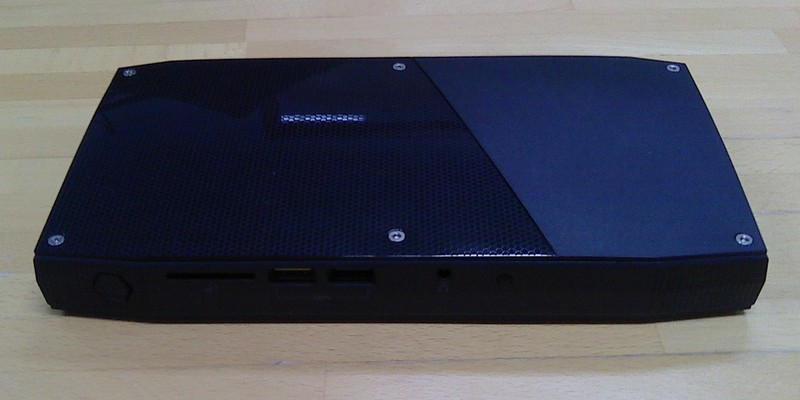
\includegraphics[height=0.14\textwidth]{pics-system/sys-comp-front.jpg} &
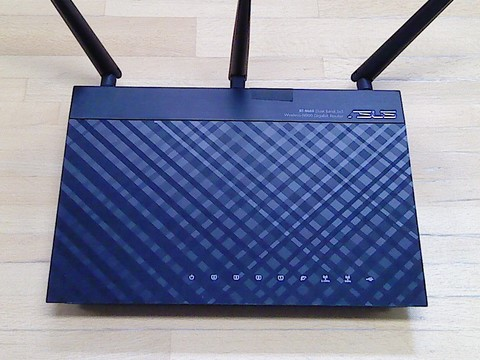
\includegraphics[height=0.14\textwidth]{pics-system/sys-router-front.jpg} &
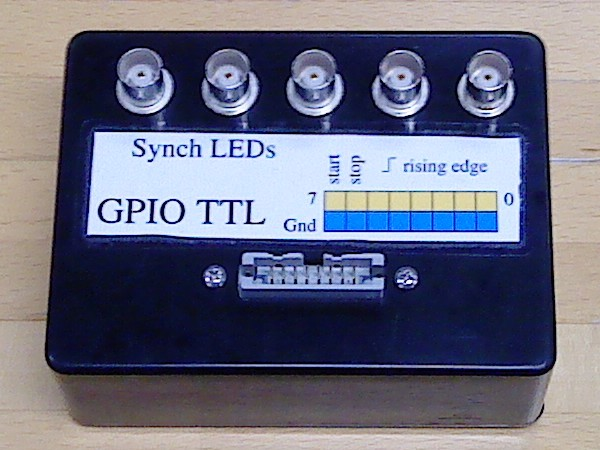
\includegraphics[height=0.14\textwidth]{pics-system/sys-gpio.jpg} &
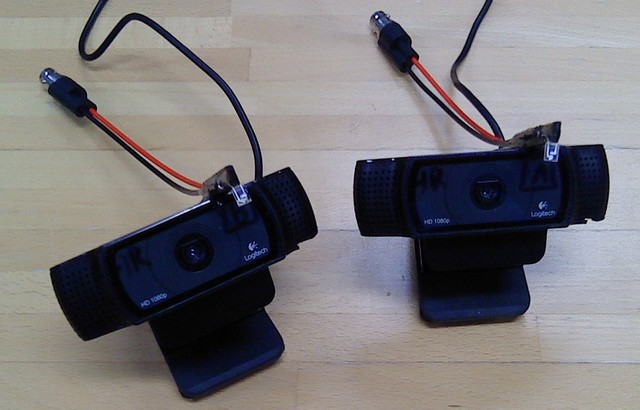
\includegraphics[height=0.14\textwidth]{pics-system/sys-cameras.jpg} \\
\end{tabular}
\end{center}

\clearpage

There are several tasks of note that have to be performed in order to
configure the NeuroCam hardware for use:

\begin{itemize}

\item The camera synchronization LEDs must be connected to the
GPIO-and-synchronization box via BNC cables.

Alternatively, a TTL-controlled lamp (visible or IR) may be placed in the
scene within view of all cameras and connected to the GPIO-and-synchronization
box.

\item The administrator password for the wireless router \textit{must} be
set to a new, stronger value. The default password (``administrator'') is
provided strictly for setup purposes.

The password for the NeuroCam network should also be changed. The default
password (``neurocam'') is easily guessed from the network name.

\item Any machines that are intended to communicate wirelessly with the
NeuroCam system must be added to the wireless router's MAC whitelist.
Machines that communicate via network cable may also need to be added,
depending on the router's configuration.

\item The game machine must be configured to stream MJPEG video, and to
respond to NeuroCam queries about offered content. The ``\verb+VLC+''
application was used for MJPEG streaming in the prototype system. Consult
VLC's documentation for further information.

Network handshaking with the game machine is described in Chapter 
\ref{handshake}.

\end{itemize}

The wireless router may be reconfigured by connecting to a wired LAN port
and accessing the web address printed on the bottom of the device.
\textbf{Do not} reset the device to factory default settings; this will lose 
all NeuroCam-related configuration.

See Chapter \ref{router} for details about configuring routers.

%
% This is the end of the file.
